\section{``Table 12'' SRFs}
%==========================
\label{app:srf.table12}
This appendix displays the "Table 12" dataset from the ATMS PFM Calibration Data Book\cite{ATMS_PFM_CalLog}, along with the ``boxcar'' SRF, based on the table \ref{tab:atms_fo_sb_and_df} data, and a representative brightness temperature spectrum.

\newpage

% Note: the "[H]" placement option is allowed due to the use of the float package
%       in the preamble. I did this to avoid the
%        ! LaTeX Error: Too many unprocessed floats.
%       error due to the large number of figures.
\begin{figure}[H]
  \centering
  \begin{tabular}{c c}
    \textsf{\textbf{(a)} Channel 1} &
    \textsf{\textbf{(b)} Channel 2} \\
    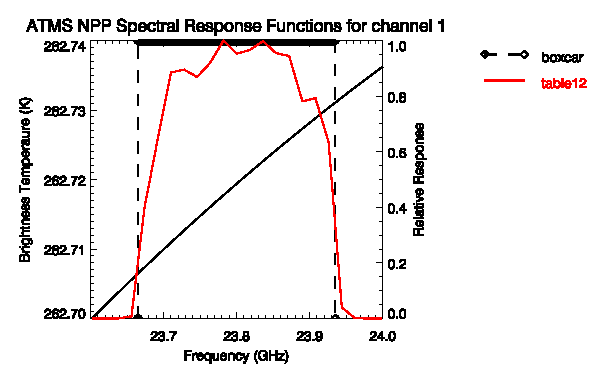
\includegraphics[bb=70 400 300 559,clip,scale=1.0]{graphics/srf/table12/atms_npp.ch1.osrf.eps} &
    \includegraphics[bb=70 400 300 559,clip,scale=1.0]{graphics/srf/table12/atms_npp.ch2.osrf.eps} \\\\

    \textsf{\textbf{(c)} Channel 3} &
    \textsf{\textbf{(d)} Channel 4} \\
    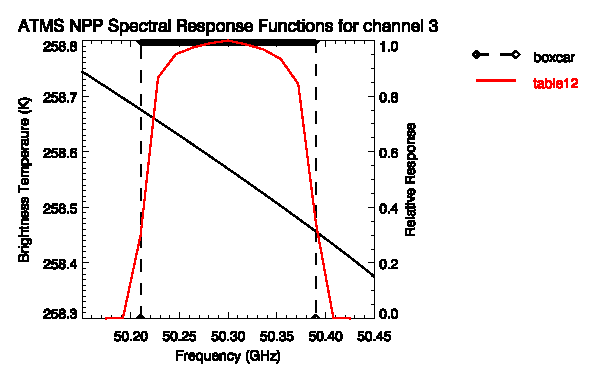
\includegraphics[bb=70 400 300 559,clip,scale=1.0]{graphics/srf/table12/atms_npp.ch3.osrf.eps} &
    \includegraphics[bb=70 400 300 559,clip,scale=1.0]{graphics/srf/table12/atms_npp.ch4.osrf.eps} \\\\

    \textsf{\textbf{(e)} Channel 5} &
    \textsf{\textbf{(f)} Channel 6} \\
    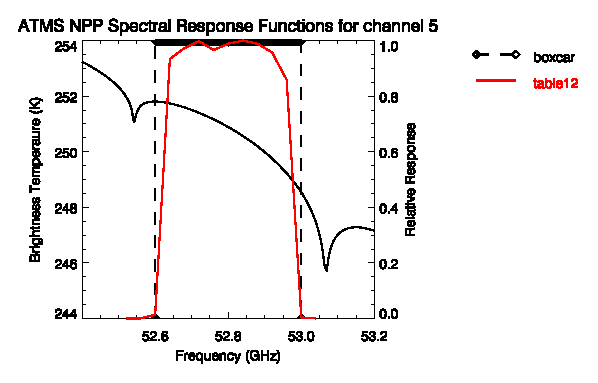
\includegraphics[bb=70 400 300 559,clip,scale=1.0]{graphics/srf/table12/atms_npp.ch5.osrf.eps} &
    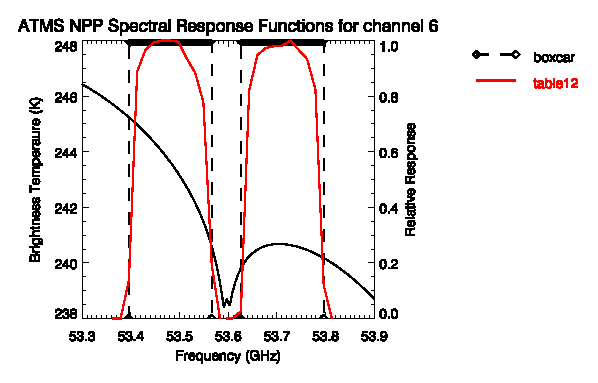
\includegraphics[bb=70 400 300 559,clip,scale=1.0]{graphics/srf/table12/atms_npp.ch6.osrf.eps}
  \end{tabular}
  \caption{Channels 1-6 of NPP ATMS Table 12 SRF data from the ATMS PFM Calibration Data Book\cite{ATMS_PFM_CalLog} with the corresponding boxcar response based on table \ref{tab:atms_fo_sb_and_df} data. A representative brightness temperature spectrum is also shown.}
  \label{fig:atms_npp.table12.ch1-6.osrf}
\end{figure}

\begin{figure}[H]
  \centering
  \begin{tabular}{c c}
    \textsf{\textbf{(a)} Channel 7} &
    \textsf{\textbf{(b)} Channel 8} \\
    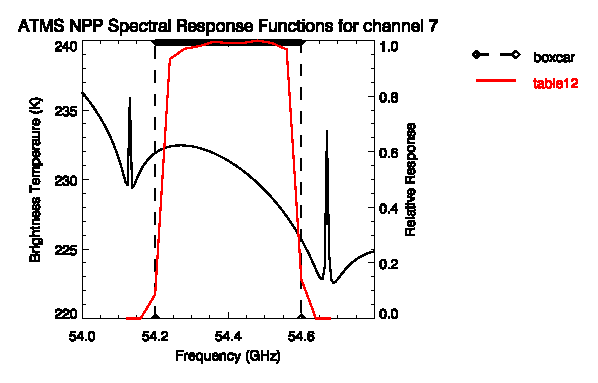
\includegraphics[bb=70 400 300 559,clip,scale=1.0]{graphics/srf/table12/atms_npp.ch7.osrf.eps} &
    \includegraphics[bb=70 400 300 559,clip,scale=1.0]{graphics/srf/table12/atms_npp.ch8.osrf.eps} \\\\

    \textsf{\textbf{(c)} Channel 9} &
    \textsf{\textbf{(d)} Channel 10} \\
    \includegraphics[bb=70 400 300 559,clip,scale=1.0]{graphics/srf/table12/atms_npp.ch9.osrf.eps} &
    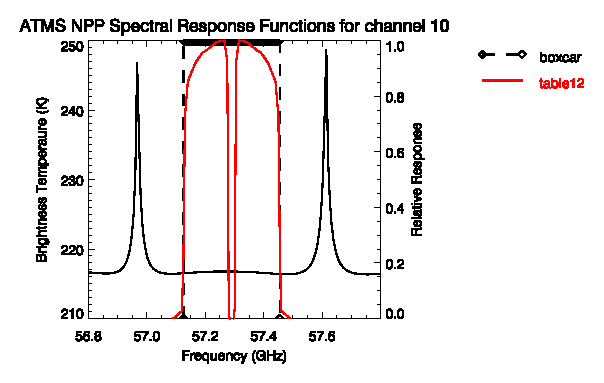
\includegraphics[bb=70 400 300 559,clip,scale=1.0]{graphics/srf/table12/atms_npp.ch10.osrf.eps} \\\\

    \textsf{\textbf{(e)} Channel 11} &
    \textsf{\textbf{(f)} Channel 12 (low $f$ passbands only)} \\
    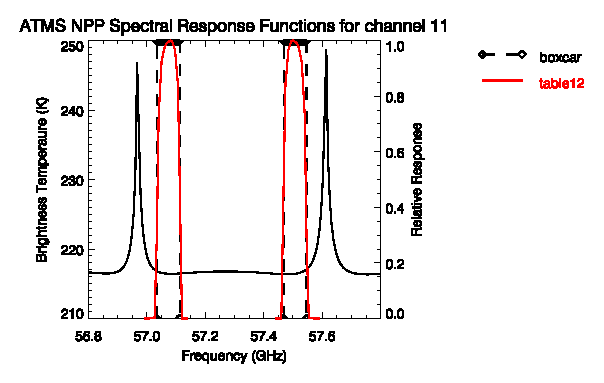
\includegraphics[bb=70 400 300 559,clip,scale=1.0]{graphics/srf/table12/atms_npp.ch11.osrf.eps} &
    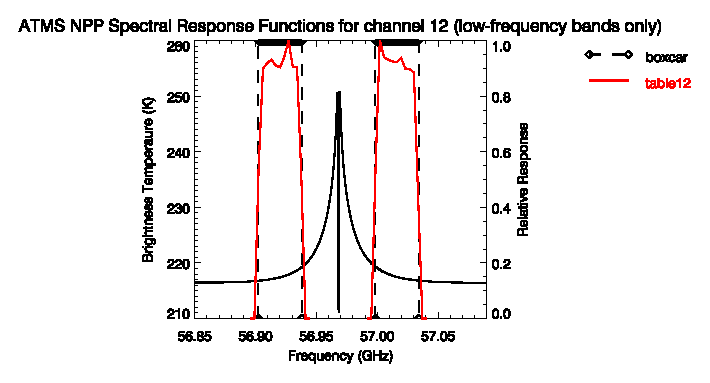
\includegraphics[bb=70 400 300 559,clip,scale=1.0]{graphics/srf/table12/atms_npp.ch12.osrf.eps}
  \end{tabular}
  \caption{Channels 7-12 of NPP ATMS Table 12 SRF data from the ATMS PFM Calibration Data Book\cite{ATMS_PFM_CalLog} with the corresponding boxcar response based on table \ref{tab:atms_fo_sb_and_df} data. A representative brightness temperature spectrum is also shown.}
  \label{fig:atms_npp.table12.ch7-12.osrf}
\end{figure}

\begin{figure}[H]
  \centering
  \begin{tabular}{c c}
    \textsf{\textbf{(a)} Channel 13 (low $f$ passbands only)} &
    \textsf{\textbf{(b)} Channel 14 (low $f$ passbands only)} \\
    \includegraphics[bb=70 400 300 559,clip,scale=1.0]{graphics/srf/table12/atms_npp.ch13.osrf.eps} &
    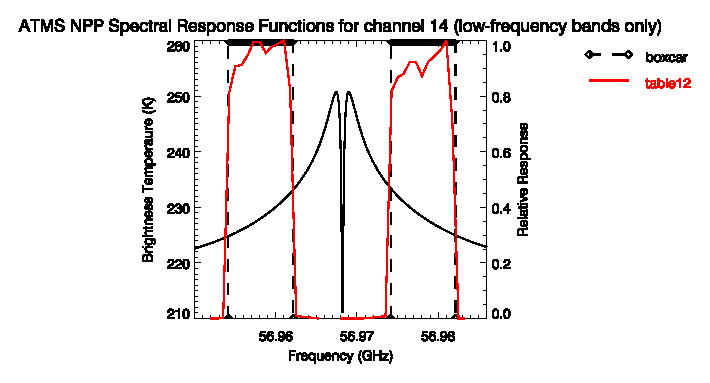
\includegraphics[bb=70 400 300 559,clip,scale=1.0]{graphics/srf/table12/atms_npp.ch14.osrf.eps} \\\\

    \textsf{\textbf{(c)} Channel 15 (low $f$ passbands only)} &
    \textsf{\textbf{(d)} Channel 16} \\
    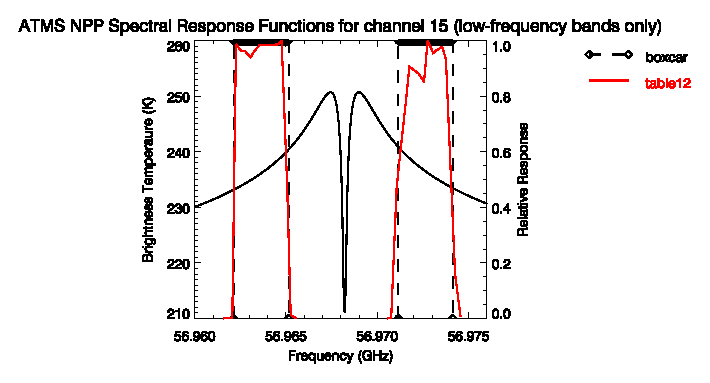
\includegraphics[bb=70 400 300 559,clip,scale=1.0]{graphics/srf/table12/atms_npp.ch15.osrf.eps} &
    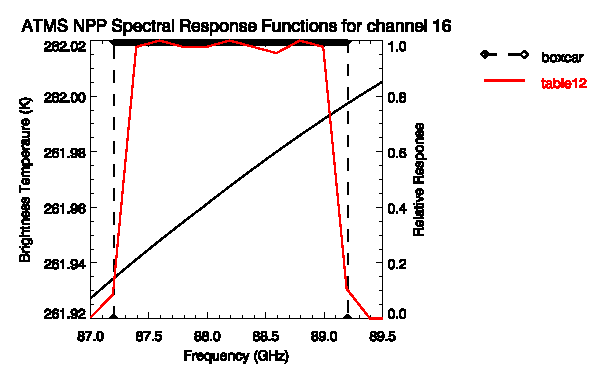
\includegraphics[bb=70 400 300 559,clip,scale=1.0]{graphics/srf/table12/atms_npp.ch16.osrf.eps} \\\\

    \textsf{\textbf{(e)} Channel 17} &
    \textsf{\textbf{(f)} Channel 18} \\
    \includegraphics[bb=70 400 300 559,clip,scale=1.0]{graphics/srf/table12/atms_npp.ch17.osrf.eps} &
    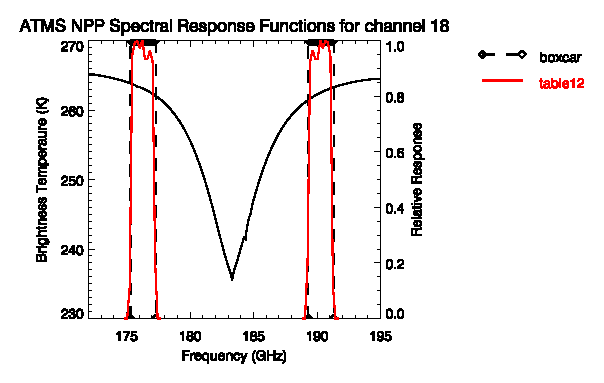
\includegraphics[bb=70 400 300 559,clip,scale=1.0]{graphics/srf/table12/atms_npp.ch18.osrf.eps}
  \end{tabular}
  \caption{Channels 13-18 of NPP ATMS Table 12 SRF data from the ATMS PFM Calibration Data Book\cite{ATMS_PFM_CalLog} with the corresponding boxcar response based on table \ref{tab:atms_fo_sb_and_df} data. A representative brightness temperature spectrum is also shown.}
  \label{fig:atms_npp.table12.ch13-18.osrf}
\end{figure}

\begin{figure}[H]
  \centering
  \begin{tabular}{c c}
    \textsf{\textbf{(a)} Channel 19} &
    \textsf{\textbf{(b)} Channel 20} \\
    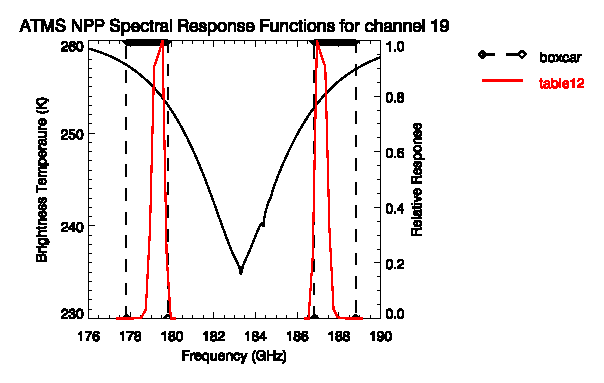
\includegraphics[bb=70 400 300 559,clip,scale=1.0]{graphics/srf/table12/atms_npp.ch19.osrf.eps} &
    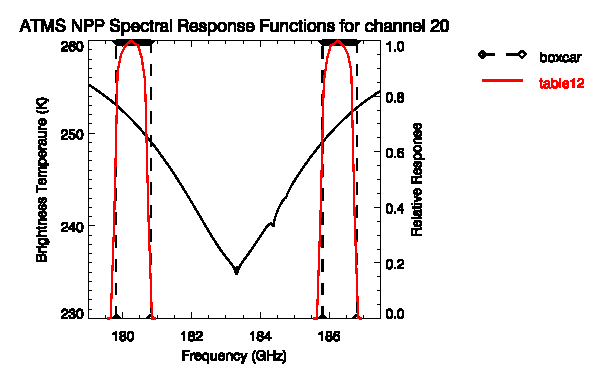
\includegraphics[bb=70 400 300 559,clip,scale=1.0]{graphics/srf/table12/atms_npp.ch20.osrf.eps} \\\\

    \textsf{\textbf{(c)} Channel 21} &
    \textsf{\textbf{(d)} Channel 22} \\
    \includegraphics[bb=70 400 300 559,clip,scale=1.0]{graphics/srf/table12/atms_npp.ch21.osrf.eps} &
    \includegraphics[bb=70 400 300 559,clip,scale=1.0]{graphics/srf/table12/atms_npp.ch22.osrf.eps}
  \end{tabular}
  \caption{Channels 19-22 of NPP ATMS Table 12 SRF data from the ATMS PFM Calibration Data Book\cite{ATMS_PFM_CalLog} with the corresponding boxcar response based on table \ref{tab:atms_fo_sb_and_df} data. A representative brightness temperature spectrum is also shown.}
  \label{fig:atms_npp.table12.ch19-22.osrf}
\end{figure}
